%!TEX program = xelatex
%!BIB program = bibtex

\documentclass[a4paper,11pt]{article}
\usepackage{graphicx}
\usepackage{amsmath, amsthm, amssymb} %better typesetting of mathematical expressions, theorems, additional symbols
\usepackage{booktabs} %fixltx2e
\usepackage[flushleft]{threeparttable}
\usepackage{tabularx}
% \usepackage[capposition=top]{floatrow}
\usepackage{caption}
% \captionsetup[measuredfigure]{labelformat=empty}
% \usepackage{bm}
% \usepackage{subcaption}
%\usepackage{epstopdf} % not supported by xelatex
% \usepackage{fullpage}
% \usepackage{enumerate}
\usepackage{authblk}
\usepackage{fontspec}
\usepackage{lscape}
\usepackage[round]{natbib} %standard package for bibliography
\usepackage{multirow}
% \usepackage[figuresleft]{rotating}
\usepackage[dvipsnames]{xcolor}
\usepackage{colortbl} % color table
\usepackage{geometry}
% \usepackage{hyperref} %hyperlink support
% \hypersetup{pdfstartview={XYZ null null 1.00},bookmarksnumbered, hypertexnames=false, colorlinks=true, linkcolor=BrickRed, citecolor=MidnightBlue, urlcolor=MidnightBlue} % zoom: default screen; numbers for bookmarks

%
%
%\usepackage{parskip}
\usepackage[nolist]{acronym}
\usepackage{longtable}
\usepackage{setspace}

\acrodef{bma}[BMA]{Bayesian Model Averaging}
\acrodef{bic}[BIC]{Bayesian Information Criterion}
\acrodef{cbf}[CBF]{Conditional Bayes Factor}
\acrodefplural{cbf}[CBFs]{Conditional Bayes Factors}
\acrodef{cswd}[CSWD]{Credit Suisse Wealth Databook}
\acrodef{gfdd}[GFDD]{Global Financial Development Database}
\acrodef{pip}[PIP]{Posterior Inclusion Probability}
\acrodefplural{pip}[PIPs]{Posterior Inclusion Probabilities}
\acrodef{fdi}[FDI]{Foreign Direct Investment}
\acrodefplural{fdi}[FDIs]{Foreign Direct Investments}
\acrodef{gdp}[GDP]{Gross Domestic Product}
\acrodef{uip}[UIP]{Unit Information Prior}
\acrodef{wb}[WB]{World Bank}
\acrodef{oecd}[OECD]{Organisation for Co-operation and Development}
\acrodef{ivbma}[IVBMA]{Instrumental Variable Bayesian Model Averaging}
\acrodef{wid}[WID]{World Inequality Database}
\acrodef{hbs}[HBS]{Household Balance Sheet}
\acrodef{uk}[UK]{United Kingdom}
\acrodef{us}[US]{United States}
\acrodef{efw}[EFW]{Economic Freedom of the World}
\acrodef{pmp}[PMP]{Posterior Model Probability}
\acrodef{wals}[WALS]{Weighted-average Least Squares}

%
%

\setlength\parindent{34pt}
\onehalfspacing
\title{Finance and Income Inequality - panel BMA approach\thanks{We thank two anonymous referees, ...}}
\author[a]{Roman Horvath}
\author[a]{Jan Mares\footnote{\footnotesize Corresponding author's address: IES FSV UK, Opletalova 26, 110 00, Praha 1; \textbf{e-mail:janxmares@gmail.com}}}
\affil[a]{Charles University, Prague}


%\renewcommand\Authands{ and }
\date{\today}

\begin{document}


\clubpenalty 9999 % no orphants (typographic properties)
\widowpenalty 9999 % no widows (typographic properties)
\def\sym#1{\ifmmode^{#1}\else\(^{#1}\)\fi} % shortcut for Stata tables

\maketitle

\thispagestyle{empty}
\begin{abstract}
    We investigate the impact of financial development on income inequality differentiating between depth, efficiency and access to financial markets and institutions. We apply panel Bayesian model averaging framework to address model uncertainty to reveal that financial development has complex influence on the income distribution within countries. The access to and efficiency of banking decrease income inequality. The size of the markets has no influence on overall income inequality, but contributes to the increasing top income shares. Moreover, unemployment along with investment into non-tangible assets increase income inequality while higher redistribution and physical capital investment imply lower levels of inequality.
\end{abstract}

\bigskip

\begin{tabular}{p{0.25\hsize}p{0.6\hsize}} %0.15
\textbf{Keywords:} & Income inequality, finance, Bayesian model averaging
\end{tabular}

\bigskip

\begin{tabular}{p{0.25\hsize}p{0.6\hsize}}
\textbf{JEL Codes:} & D31, E21\\
\end{tabular}

\clearpage
\setcounter{page}{1}

\section{Introduction}
% \label{sec:intro}

\section{Related literature}
% \label{sec:literature}


\citet{pikettyandzucman2014}
\citet{van2018inequality} provide evidence that income inequality in the \ac{us} has different implications for the future income growth of the rich and the poor. High inequality seems to hurt the prospects of the poor while the top of the distribution is unaffected. The rich thus disproportianately benefit from higher inequality as their subsequent income exhibit faster growth. The authors attribute this effect to the political channel the rich use to lobby in favour of the policies which support their economic interests. Preferences of the rich are ultimately more likely to determine public policy than the preferences of the majority \citep{gilens_page_2014}. High inequality together with a credit constraint and rich driving the political process results in low government spending and lasting inequality.

\citet{marrero2013inequality} introduce two types of inequality - inequality of opportunity and inequality of effort/luck. Applying this to the EU countries and US states, they show that inequality of opportunity (driven by race and parental education ...) is negatively related to growth while the residual "good" inequality is growth inducing.

Income inequality and growth may intersect through varying channels. Accumulation of savings, unobservable effort, and investment project size favour the prediction on growth inducing inequality. Negative impact of inequality on human capital accumulation, entrepreneurial activity, and hence growth provides argument for the opposing view.

The average income inequality rose across \ac{oecd} by 1.4 percentage points \citep{oecd2013crisis}.

\citet{LawSingh2014} argue that financial development decrease income inequality by allowing the poor to invest in human and physical capital.

\citet{nolan2019drivers} bring a survey of the literature on determinants of inequality, summarizing the complexity of the inequality dynamics. They stress that many of the determinants are interlinked which implies difficulty in assigning precise effects to individual drivers of inequality. Additionally, they encourage complementary individual country case studies to support the finding of the general cross-country estimates.

\subsection{theory}
\citet{galormoav2004} provide a theoretical framework of thinking about the link between income inequality and financial development. In their model, the income inequality falls due to the decrease of financial friction which allows for physical and human capital accumulation of the poor. That is the extensive margin of financial development at work.

\citet{banerjeenewman1990} also offer a theoretical setup in favour of the capital accumulation hypothesis due to finance (liberalization as claimed by \citet{de2017finance}) and inequality decreasing effect.

\citet{GreenwoodJovanovic1990} on the contrary present a model where the intensive margin of the financial development is the key force and the benefits of more finance are accrued by the incumbents - primarilly the rich - which implies an inequality increasing effect.

An exemption from focus solely on the size of financial sector is the study by \citet{naceurzhang2016} which applies a similar approach to ours, taking into consideration the access, efficiency, and stability of the financial sector. However, there are severe limitation to their study. First, their coverarage does not correspond to the availability of the data. Second, they do not account for the different dimensions of finance simultaneously and always use a single indicator of development at a time. Third, they do not explicitly differentiate between the banking sector and financial markets. We provide a more detailed as well as more robust picture of the financial development effect on finance in these dimensions.

\citet{gwartney2017} provide an economic freedom index of the Fraser Institute.

\citet{de2017finance} examine different dimensions of finance on income inequality. Their results suggest that financial development, financial liberalization, and banking crises all increase market income inequality within countries. Additionally, they show that the effect of financial liberalization is conditional on democratic accountability. The higher the accountability, the less severe is the negative impact of liberalization on inequality. On the contrary, the financial development, proxied by the credit to GDP ratio, has inequality increasing effect irrespective of the institutional background.

\citet{claessens2007finance} explore the connectedness of growth, finance, and inequality, stressing the importance of institutional background in the effects.  

\citet{perotti2007investor} present a theoretical framework how established interests lobby for lower investor protection to prevent entrance of the new competitors. Greater accountability of the politicians is reflected in higher bribe required from teh lobbyist therefore higher accountability implies higher market entry on more competition. After confirming their prediction empirically, they show that the most important factor of accountability is not the formal measure of democratic institutions, but \emph{newspaper readership} which they interpret as broad awareness of policy choices and their outcomes.

Summary of the theoretical preditions in \citet{demirgucc2009finance} on pages 20-23 for the review.

\citet{furceri2019robust} apply \ac{wals} to identify robust determinants of income inequality. They are the closest paper to ours since they account for model uncertainty in the estimation. Their focus if more general rathar than on finance specifically. Out work offers more detailed contribution in terms of the role of finance in shaping income inequality. On the top of that, we differ from their analysis by examining multiple measures of inequality and specifically identifying the determinants of top income shares along with the determinants of the overall income distribution represented by income Gini index. We provide further evidence in all these dimensions.

\section{Data}
% \label{sec:data}
\begin{figure}
    \caption{Gini Coefficient and Efficiency of Financial Institutions}
    \label{fig:ginifie}
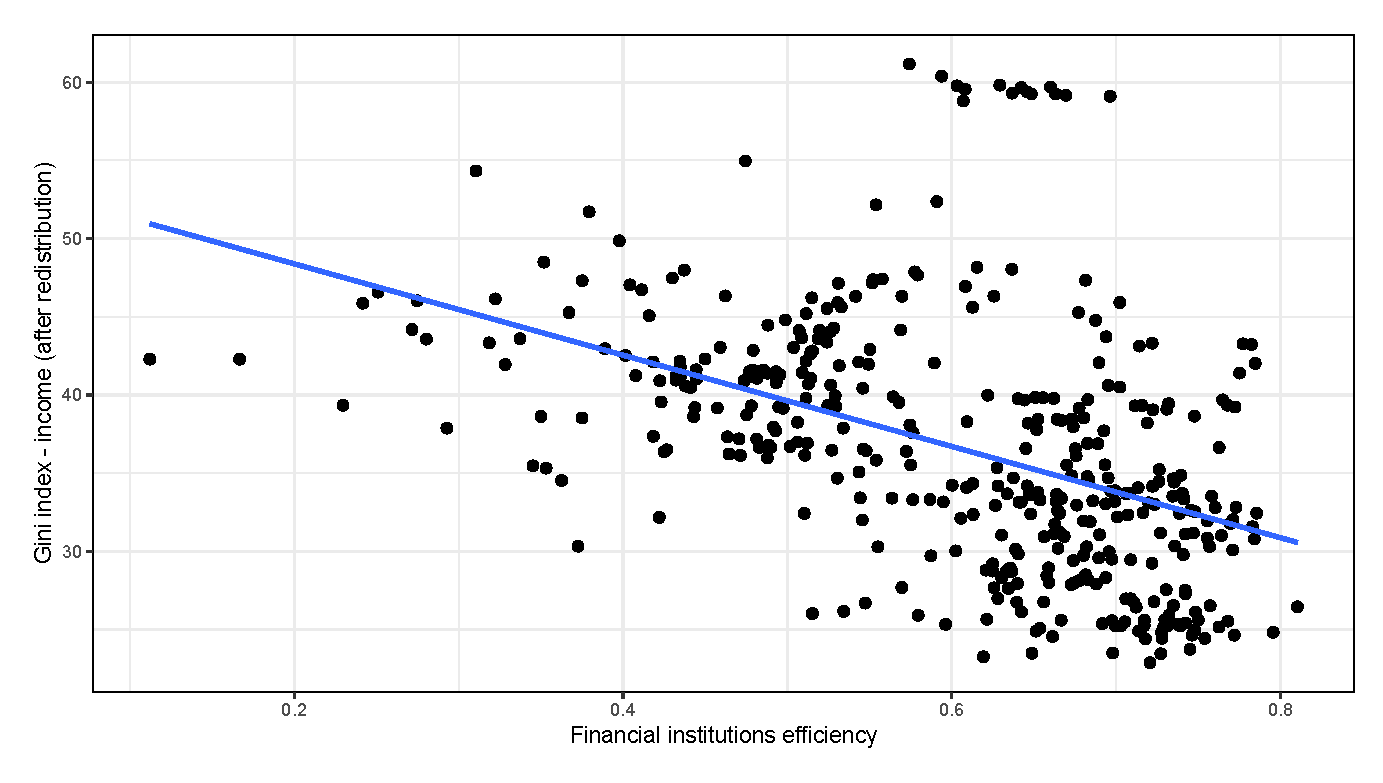
\includegraphics[width=\textwidth, keepaspectratio]{figures/FIEGiniNet}
\end{figure}

\begin{figure}
    \caption{Gini Coefficient and Access to Financial Institutions}
    \label{fig:ginifia}
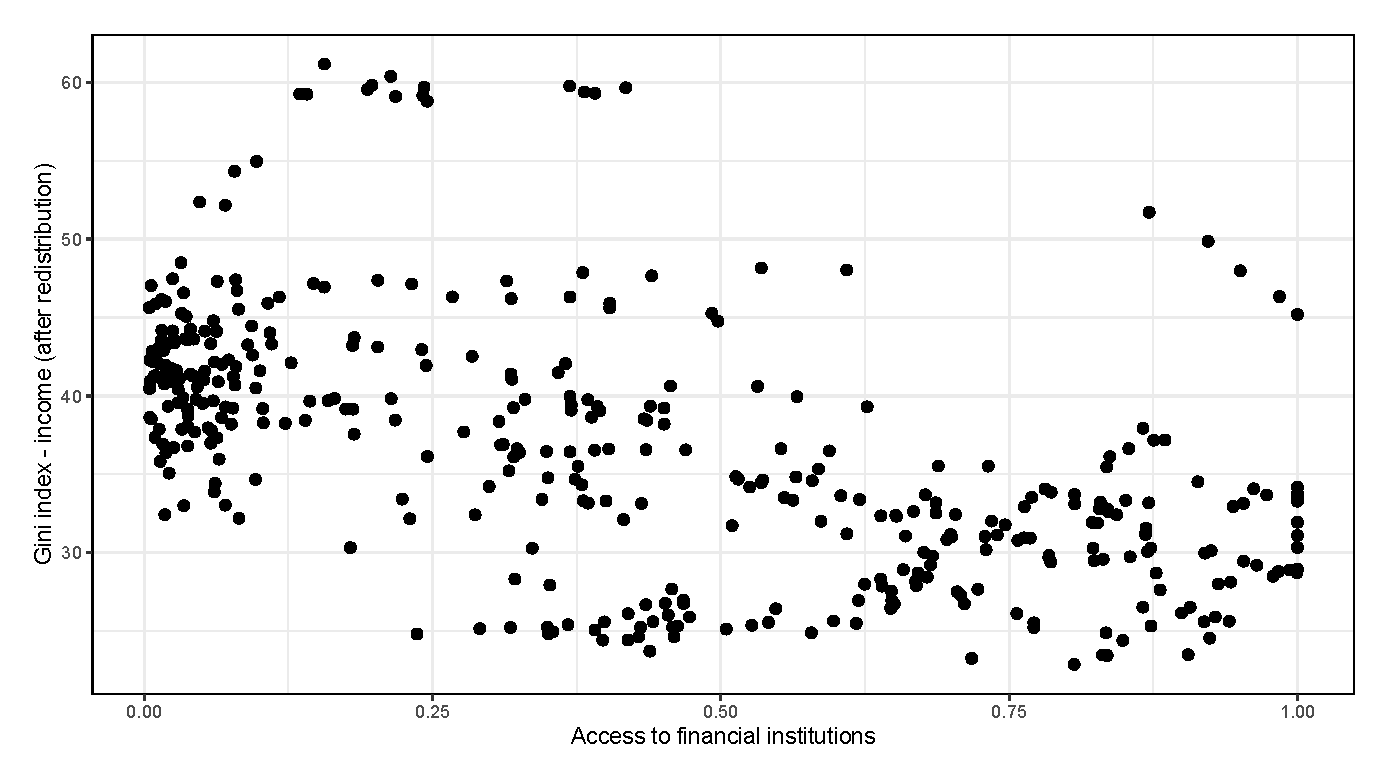
\includegraphics[width=\textwidth, keepaspectratio]{figures/FIAGiniNet}
\end{figure}

\begin{figure}
    \caption{Gini Coefficient and Depth of Financial Institutions}
    \label{fig:ginifid}

\includegraphics[width=\textwidth, keepaspectratio]{figures/FIDGiniNet}
\end{figure}

\begin{figure}
    \caption{Gini Coefficient and Depth of Financial Markets}
    \label{fig:ginifmd}
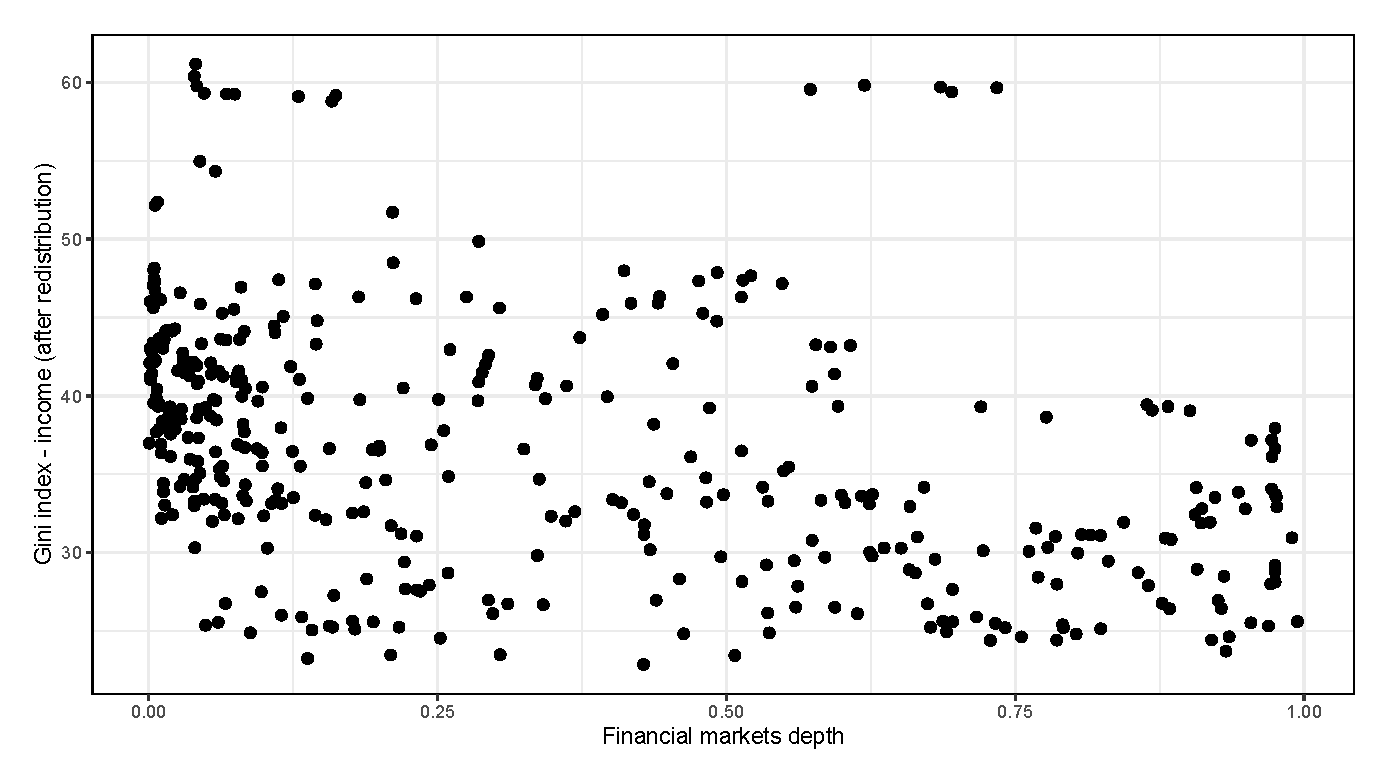
\includegraphics[width=\textwidth, keepaspectratio]{figures/FMDGiniNet}
\end{figure}

\begin{figure}
    \caption{Gini Coefficient and Government Expenditures}
    \label{fig:ginigovexp}
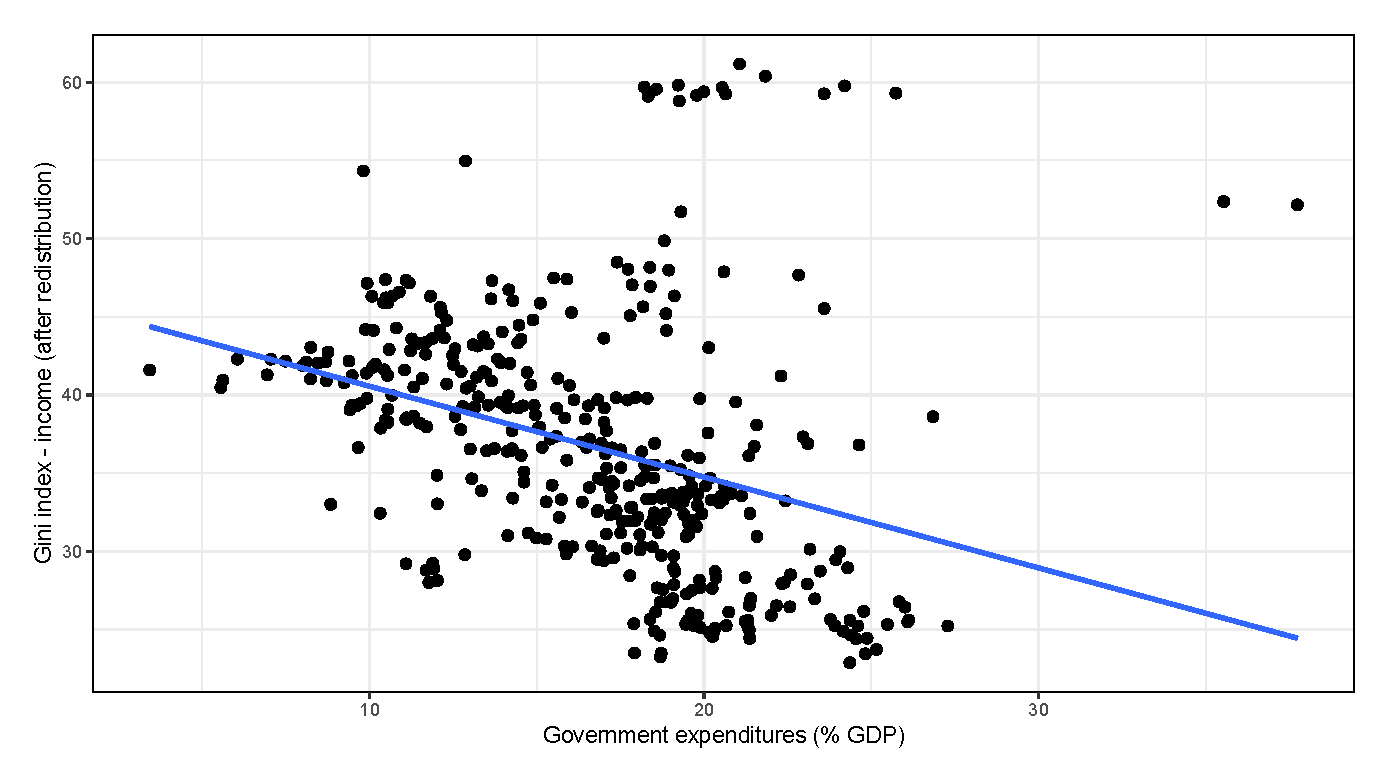
\includegraphics[width=\textwidth, keepaspectratio]{figures/GovExpGiniNet}
\end{figure}

\begin{figure}
    \caption{Gini Coefficient and Mortality}
    \label{fig:ginimort}
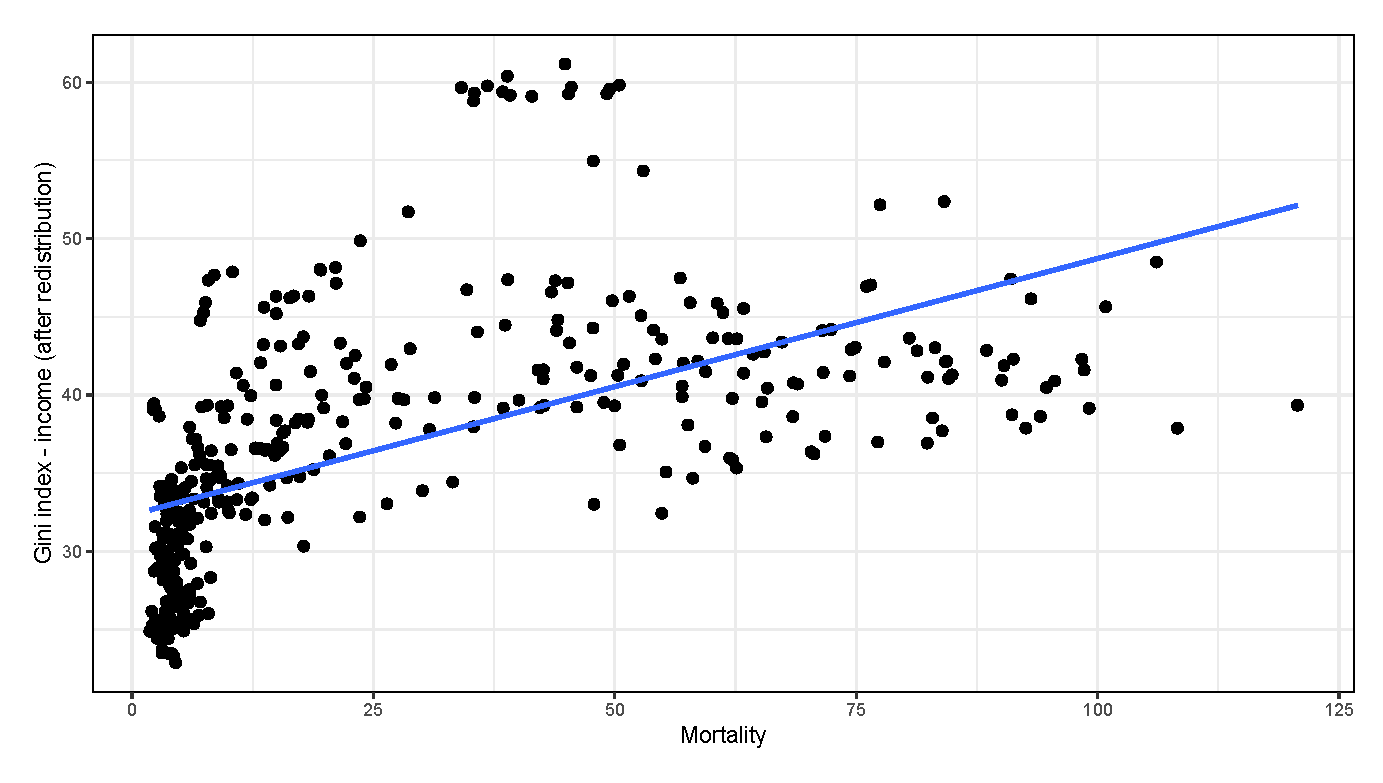
\includegraphics[width=\textwidth, keepaspectratio]{figures/MortGiniNet}
\end{figure}

\begin{figure}
    \caption{Gini Coefficient and \ac{gdp} per capita}
    \label{fig:ginigdp}
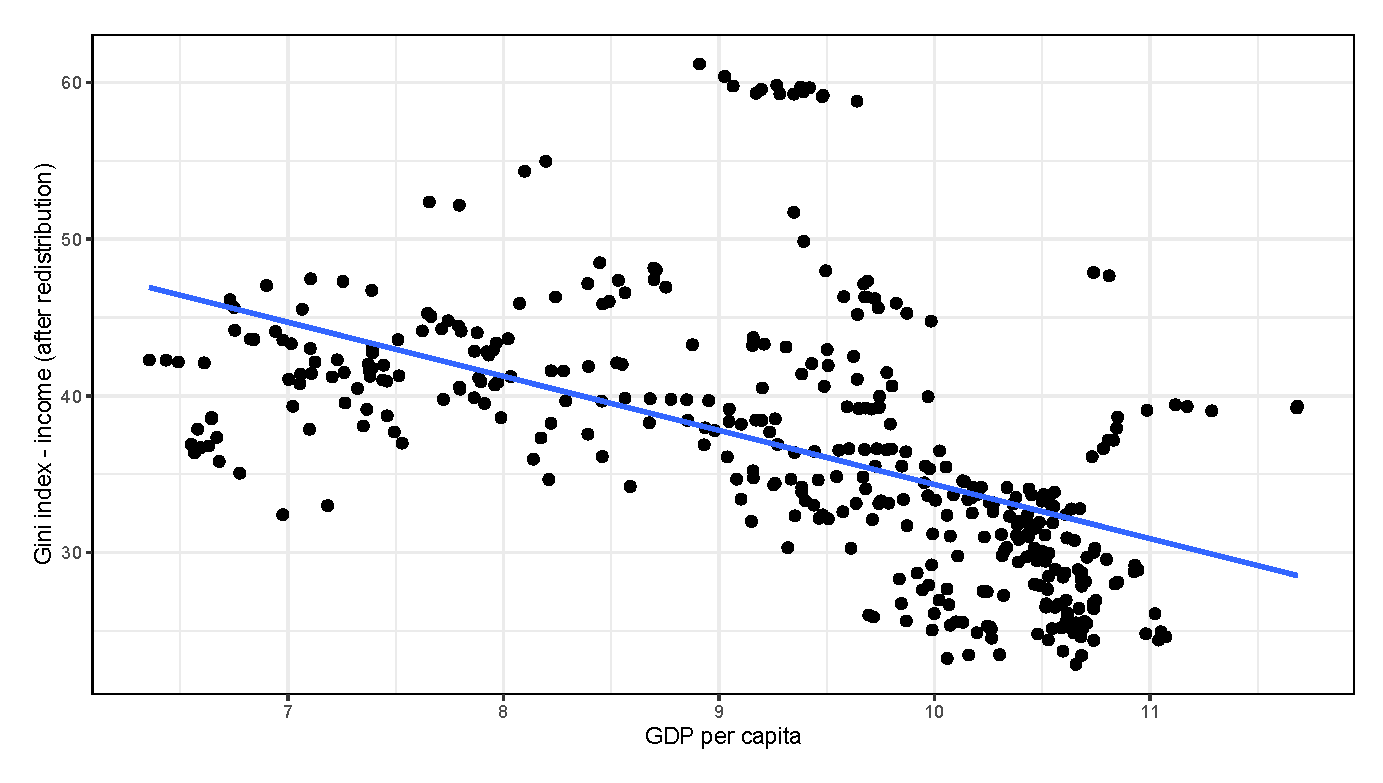
\includegraphics[width=\textwidth, keepaspectratio]{figures/GDPGiniNet}
\end{figure}

\begin{figure}
    \caption{Gini Coefficient and Rule of Law}
    \label{fig:ginirule}

\includegraphics[width=\textwidth, keepaspectratio]{figures/RuleLawGiniNet}
\end{figure}

\begin{figure}
    \caption{Gini Coefficient and Inflation}
    \label{fig:giniinfl}
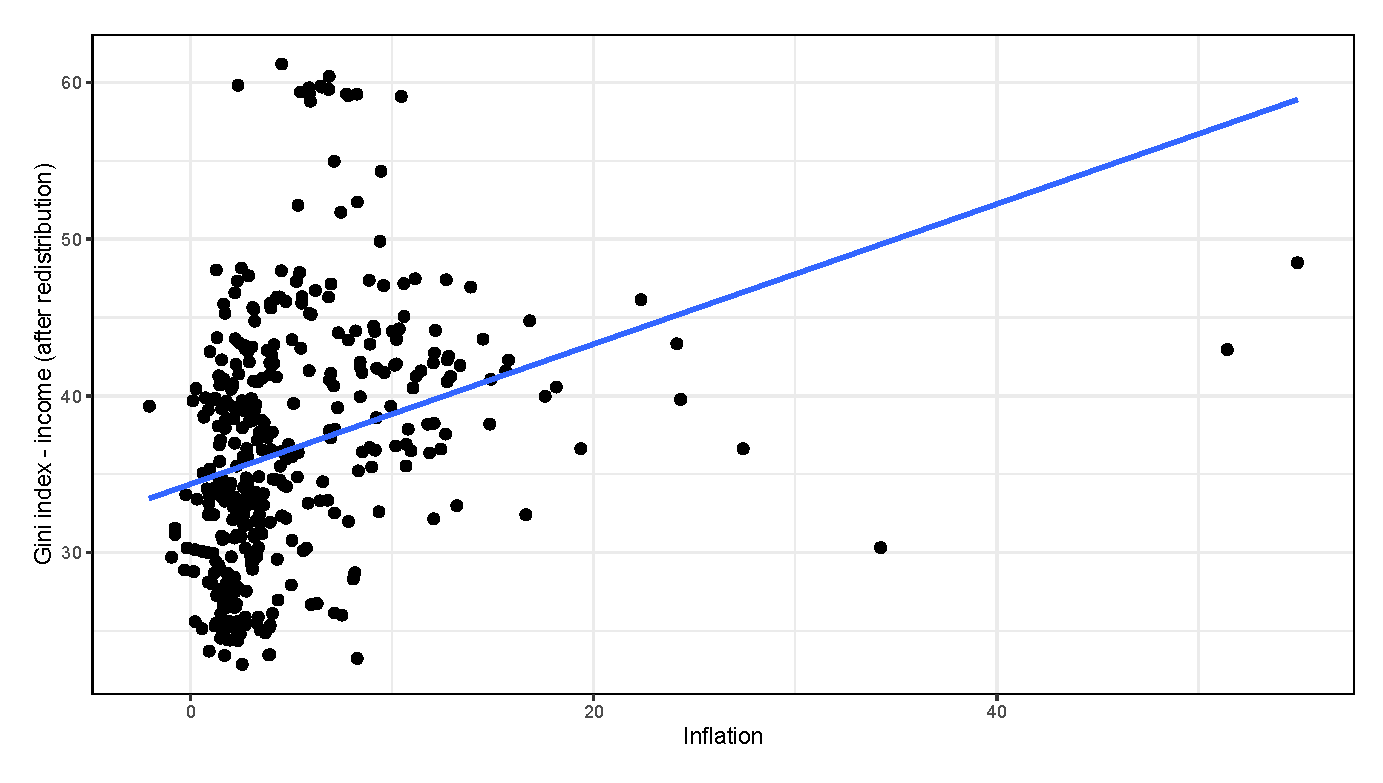
\includegraphics[width=\textwidth, keepaspectratio]{figures/InflGiniNet}
\end{figure}

\begin{figure}
    \caption{Gini Coefficient and Equipment Investment}
    \label{fig:giniequipi}

\includegraphics[width=\textwidth, keepaspectratio]{figures/EquipIGiniNet}
\end{figure}

\begin{figure}
    \caption{Gini Coefficient and Trade Openness}
    \label{fig:ginitrade}

\includegraphics[width=\textwidth, keepaspectratio]{figures/TradeOpenGiniNet}
\end{figure}

\begin{figure}
    \caption{Gini Coefficient and Financial Development Indicators}
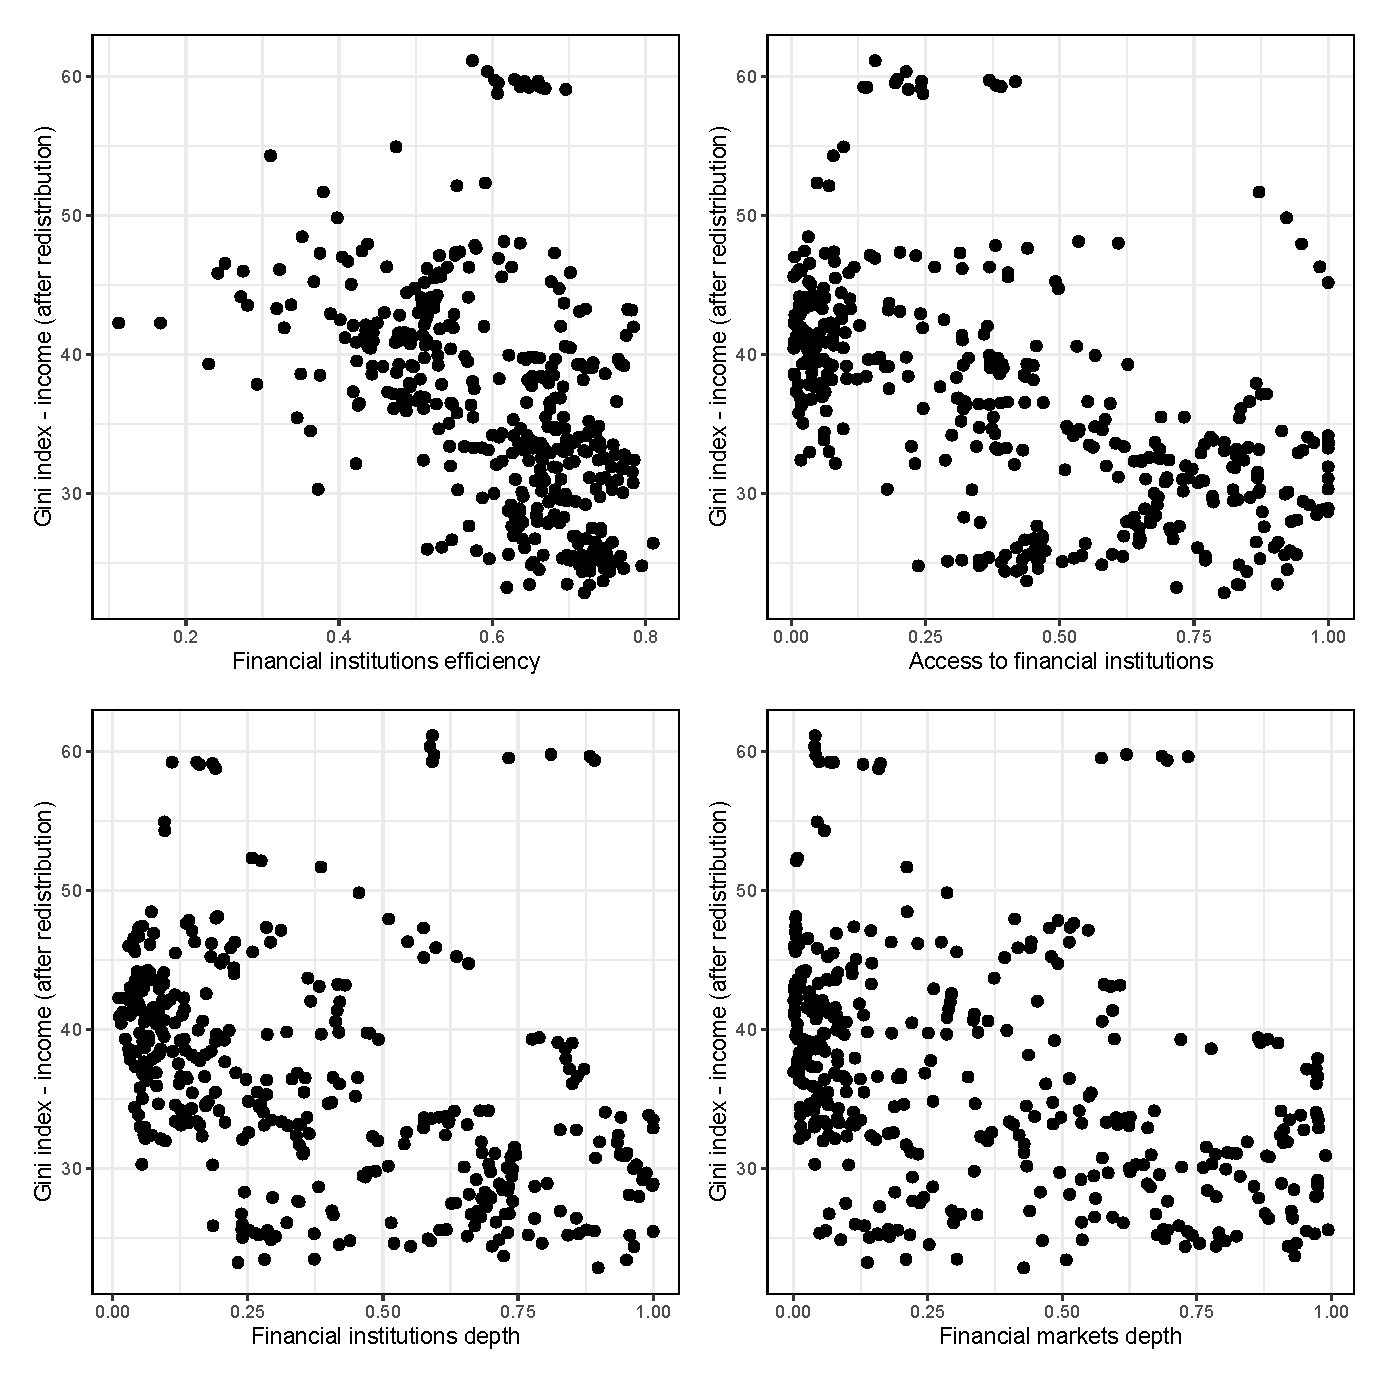
\includegraphics[width=\textwidth, keepaspectratio]{figures/plots_findev_gini}
\end{figure}

%
%

\begin{figure}
    \caption{Gini Coefficient and Efficiency of Financial Institutions}
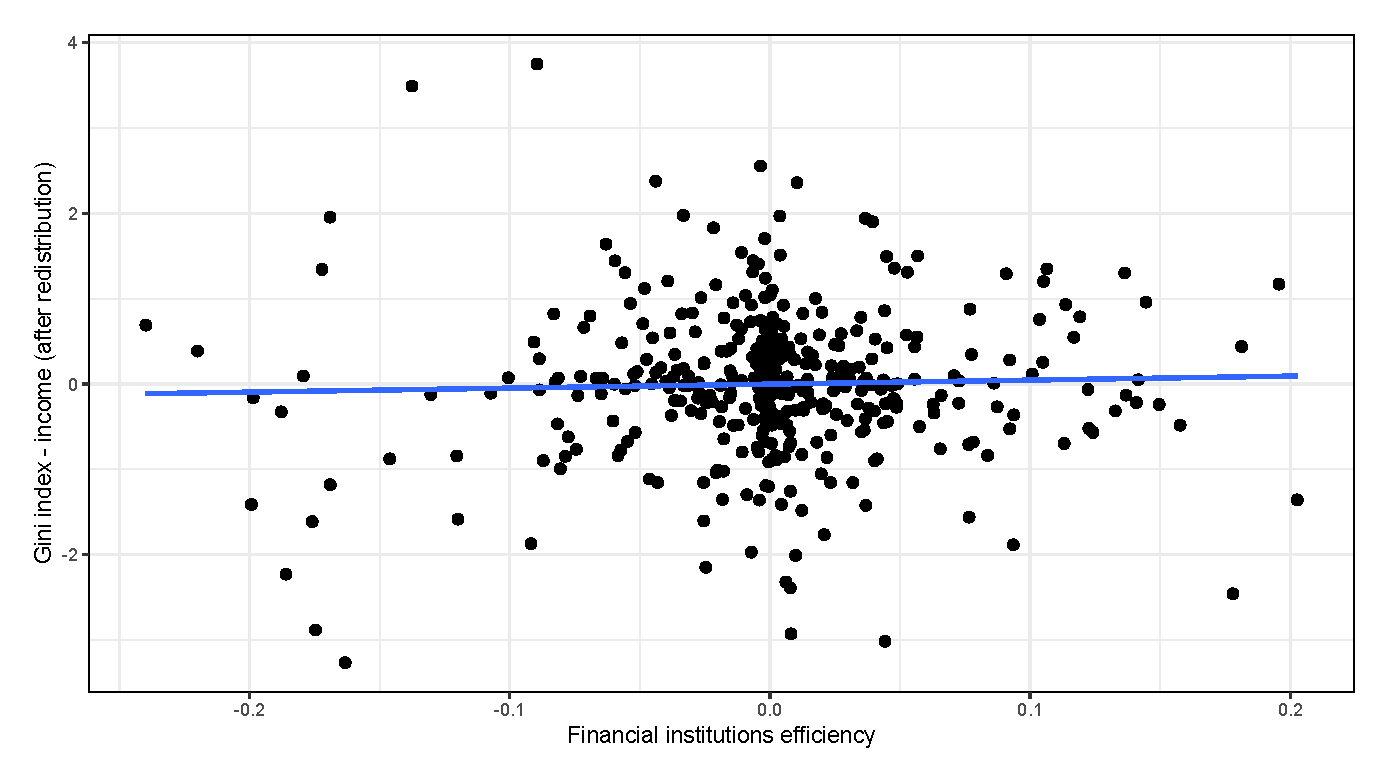
\includegraphics[width=\textwidth, keepaspectratio]{figures/FIEGiniNet_dm}
\end{figure}

\begin{figure}
    \caption{Gini Coefficient and Access to Financial Institutions}
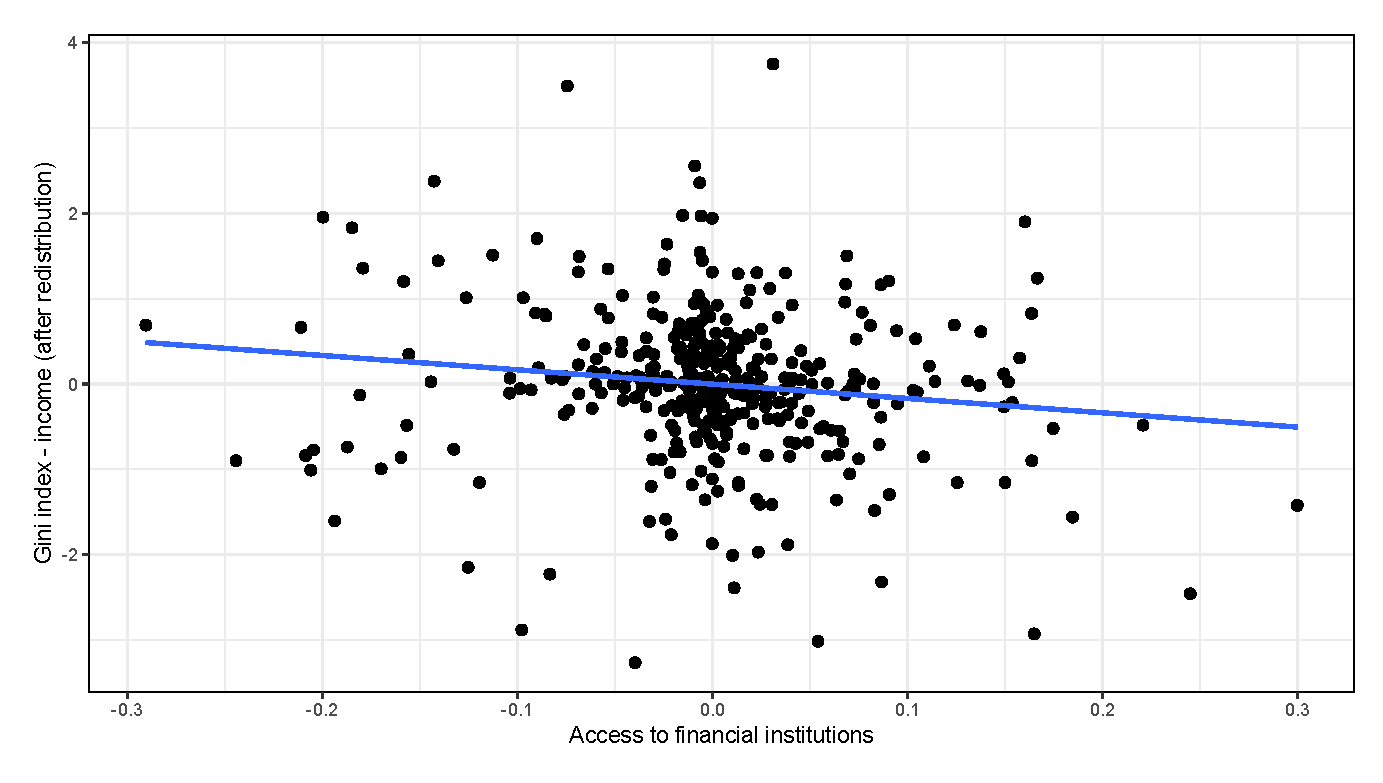
\includegraphics[width=\textwidth, keepaspectratio]{figures/FIAGiniNet_dm}
\end{figure}

\begin{figure}
    \caption{Gini Coefficient and Depth of Financial Institutions}
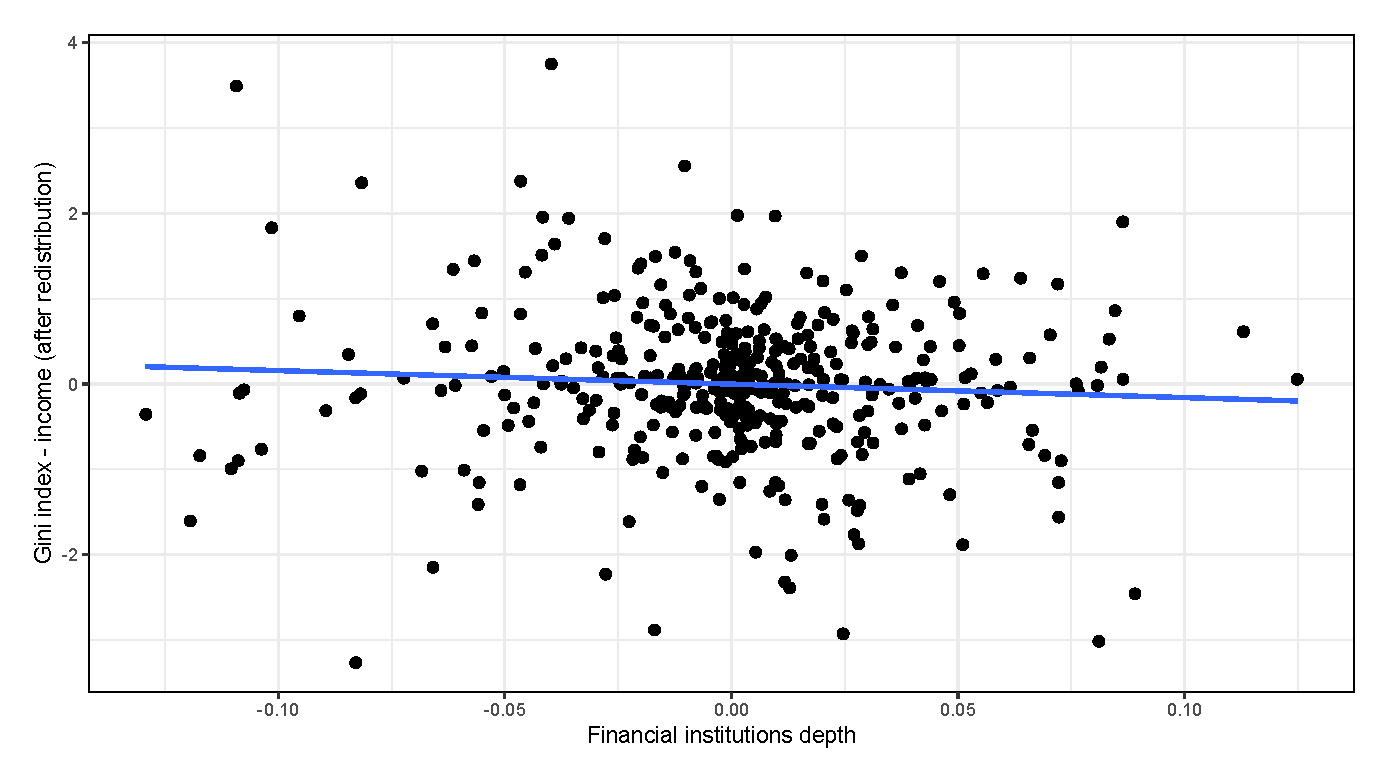
\includegraphics[width=\textwidth, keepaspectratio]{figures/FIDGiniNet_dm}
\end{figure}

\begin{figure}
    \caption{Gini Coefficient and Depth of Financial Markets}
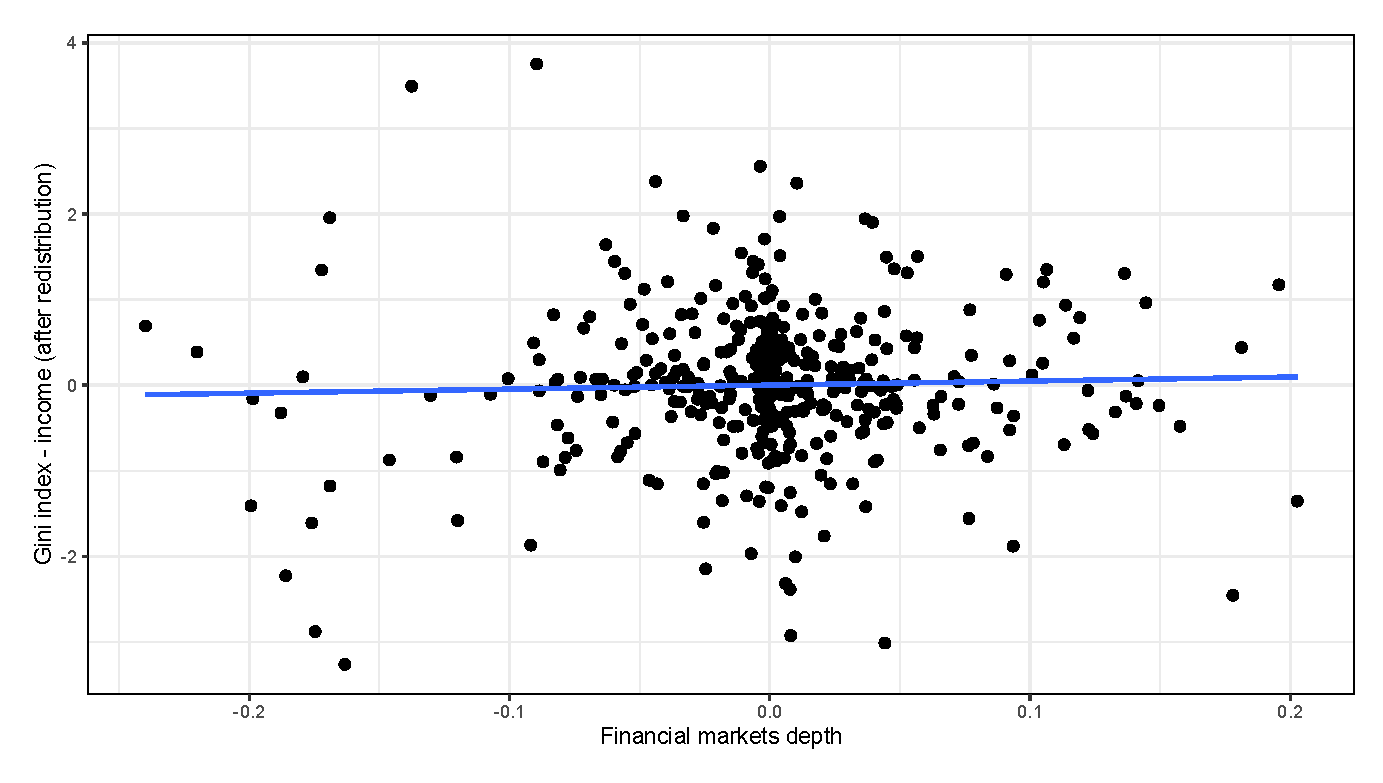
\includegraphics[width=\textwidth, keepaspectratio]{figures/FMDGiniNet_dm}
\end{figure}

\begin{figure}
    \caption{Gini Coefficient and Government Expenditures}
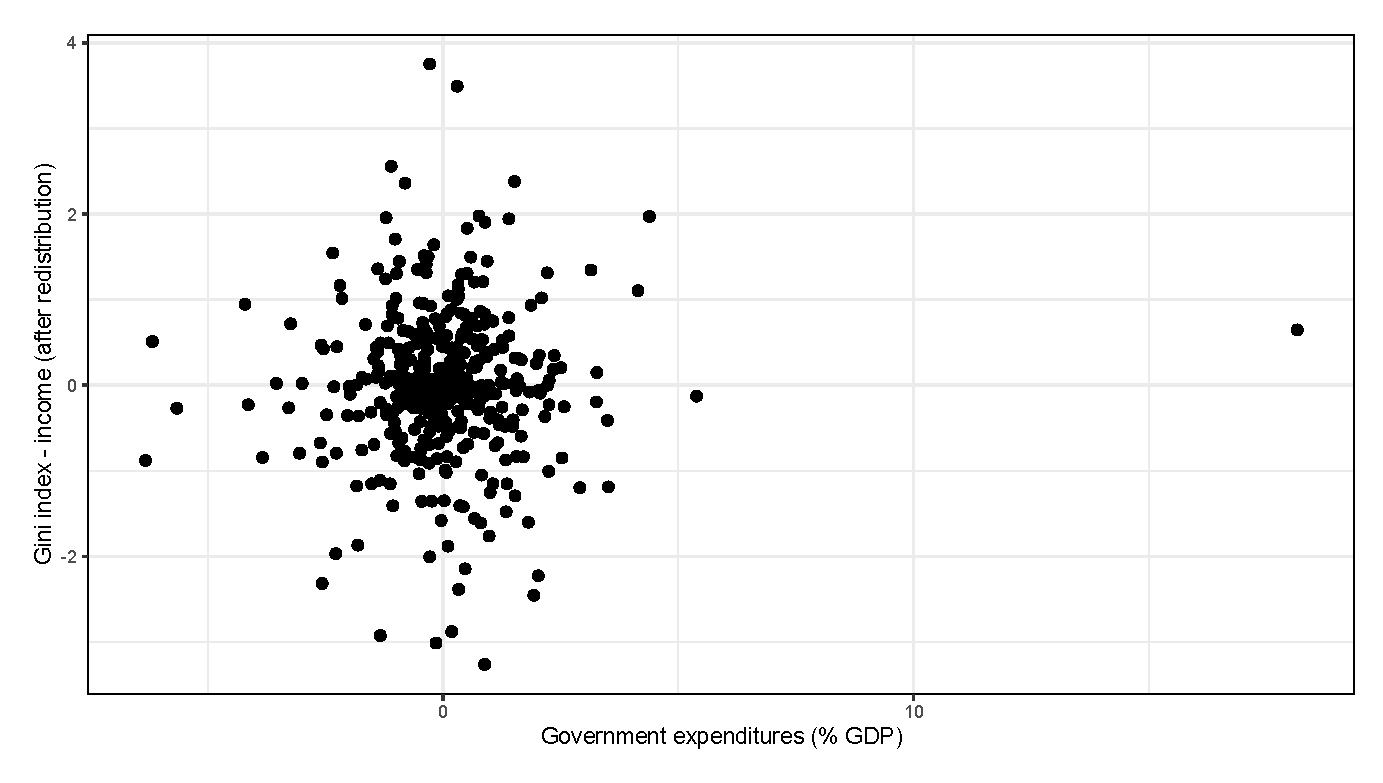
\includegraphics[width=\textwidth, keepaspectratio]{figures/GovExpGiniNet_dm}
\end{figure}

\begin{figure}
    \caption{Gini Coefficient and Mortality}
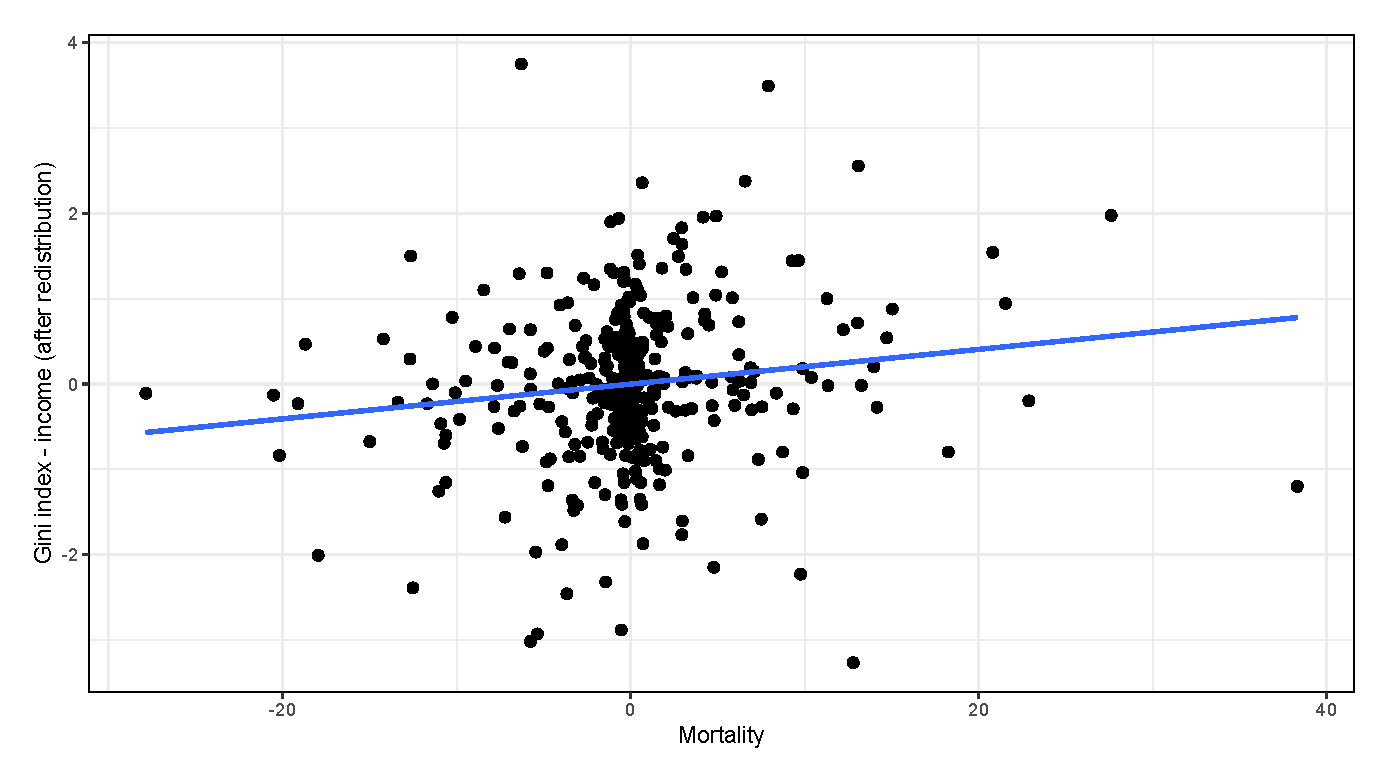
\includegraphics[width=\textwidth, keepaspectratio]{figures/MortGiniNet_dm}
\end{figure}

\begin{figure}
    \caption{Gini Coefficient and \ac{gdp} per capita}
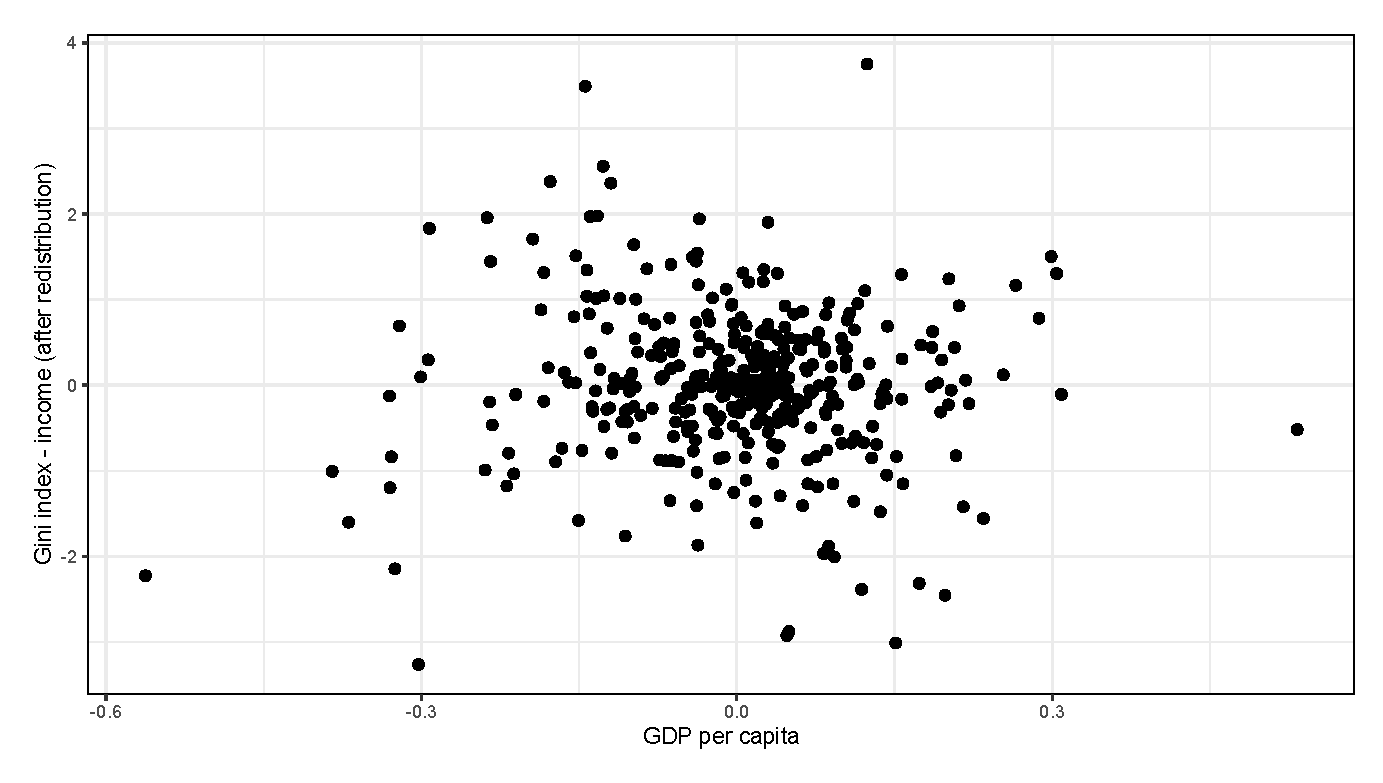
\includegraphics[width=\textwidth, keepaspectratio]{figures/GDPGiniNet_dm}
\end{figure}

\begin{figure}
    \caption{Gini Coefficient and Rule of Law}
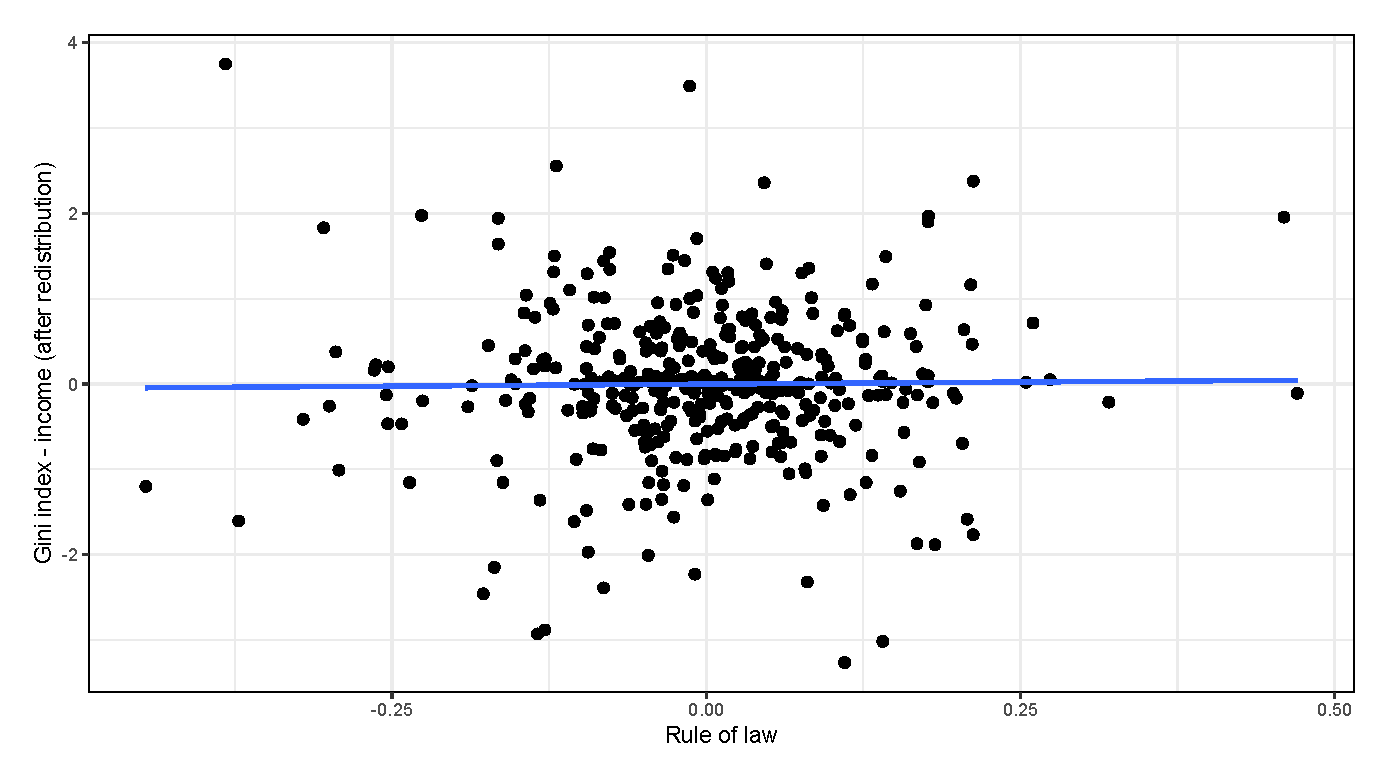
\includegraphics[width=\textwidth, keepaspectratio]{figures/RuleLawGiniNet_dm}
\end{figure}

\begin{figure}
    \caption{Gini Coefficient and Inflation}
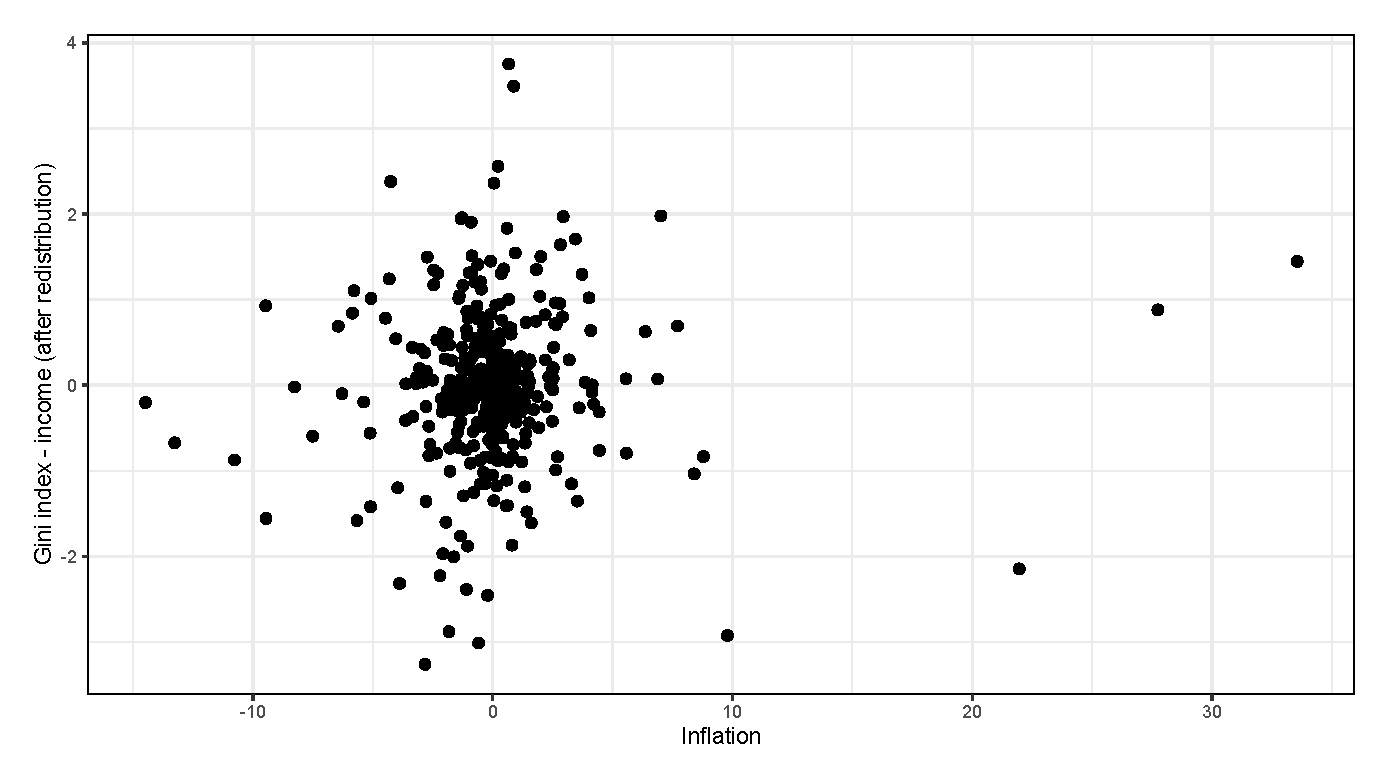
\includegraphics[width=\textwidth, keepaspectratio]{figures/InflGiniNet_dm}
\end{figure}

\begin{figure}
    \caption{Gini Coefficient and Equipment Investment}
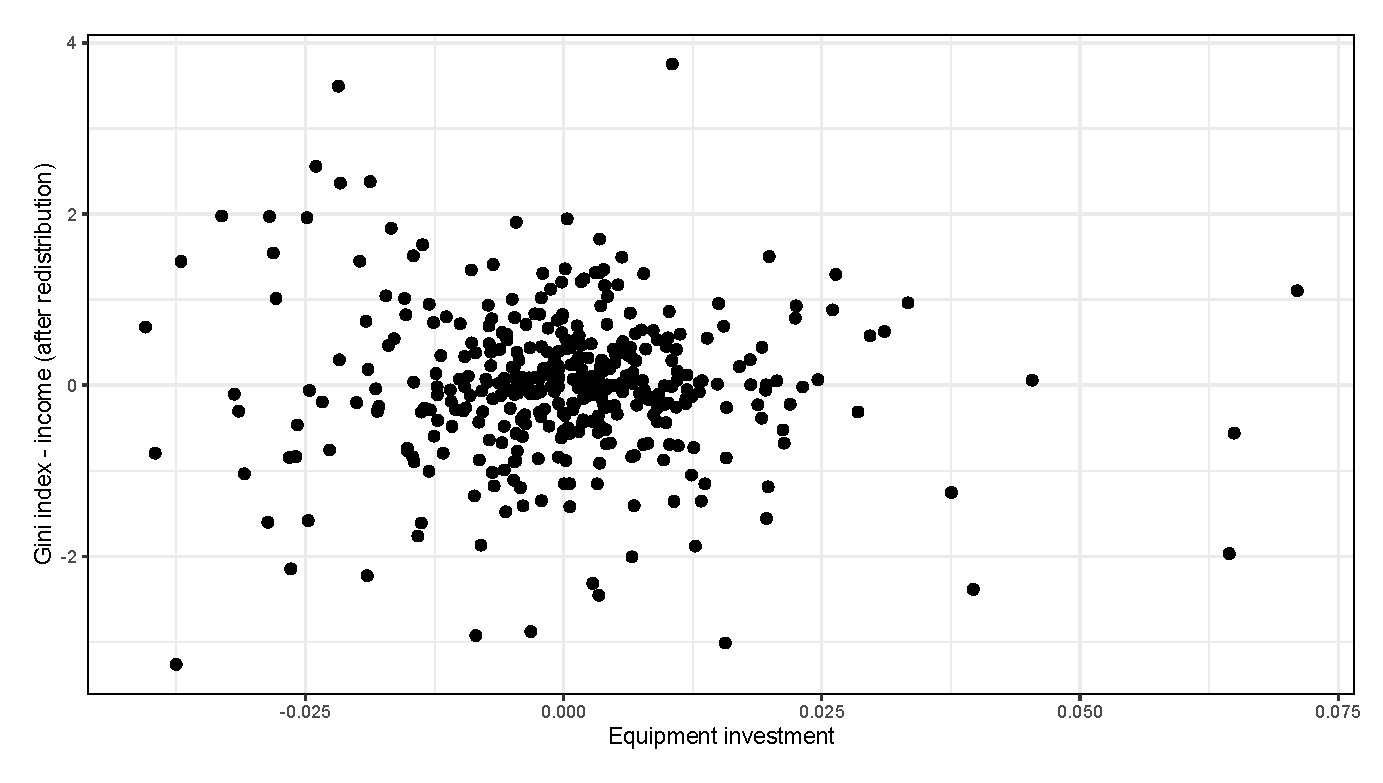
\includegraphics[width=\textwidth, keepaspectratio]{figures/EquipIGiniNet_dm}
\end{figure}

\begin{figure}
    \caption{Gini Coefficient and Trade Openness}
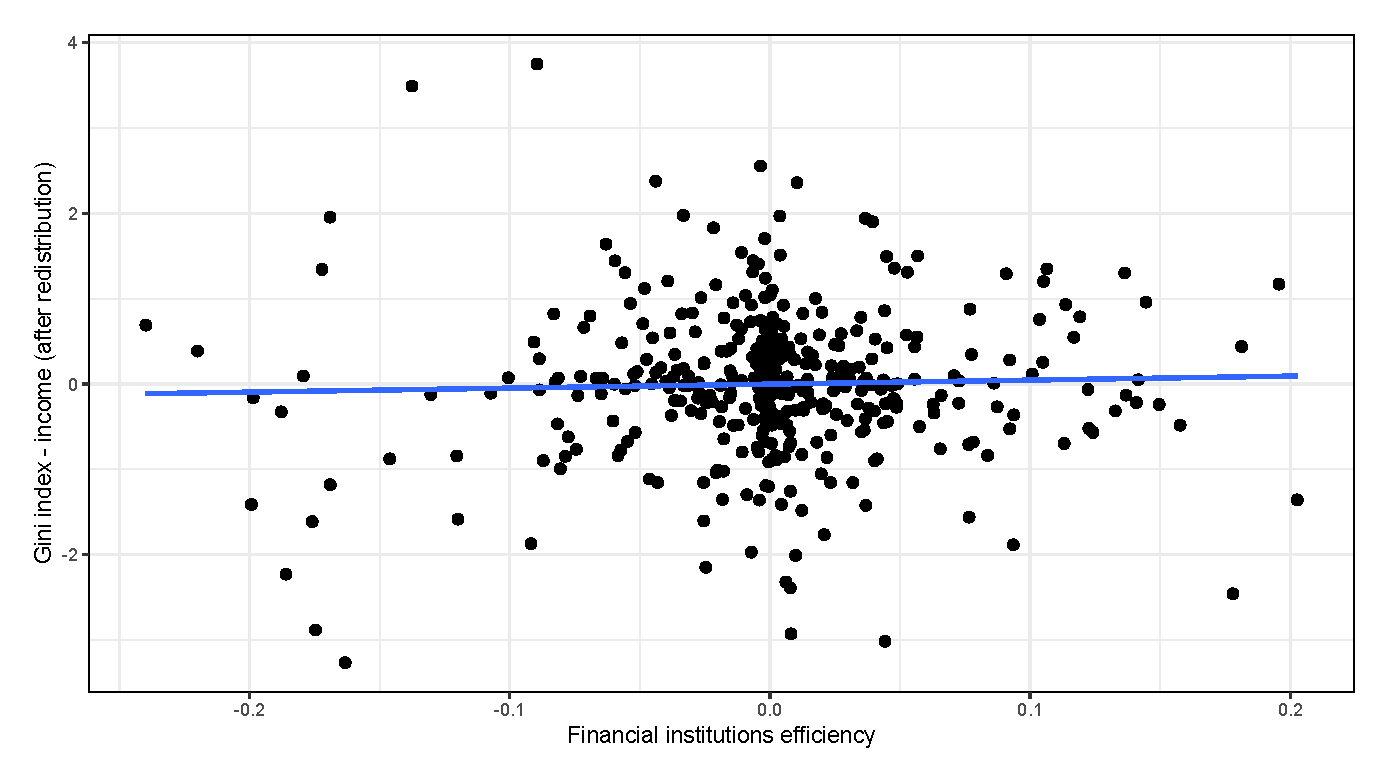
\includegraphics[width=\textwidth, keepaspectratio]{figures/TradeOpenGiniNet_dm}
\end{figure}

\begin{figure}
    \caption{Gini Coefficient and Financial Development Indicators}
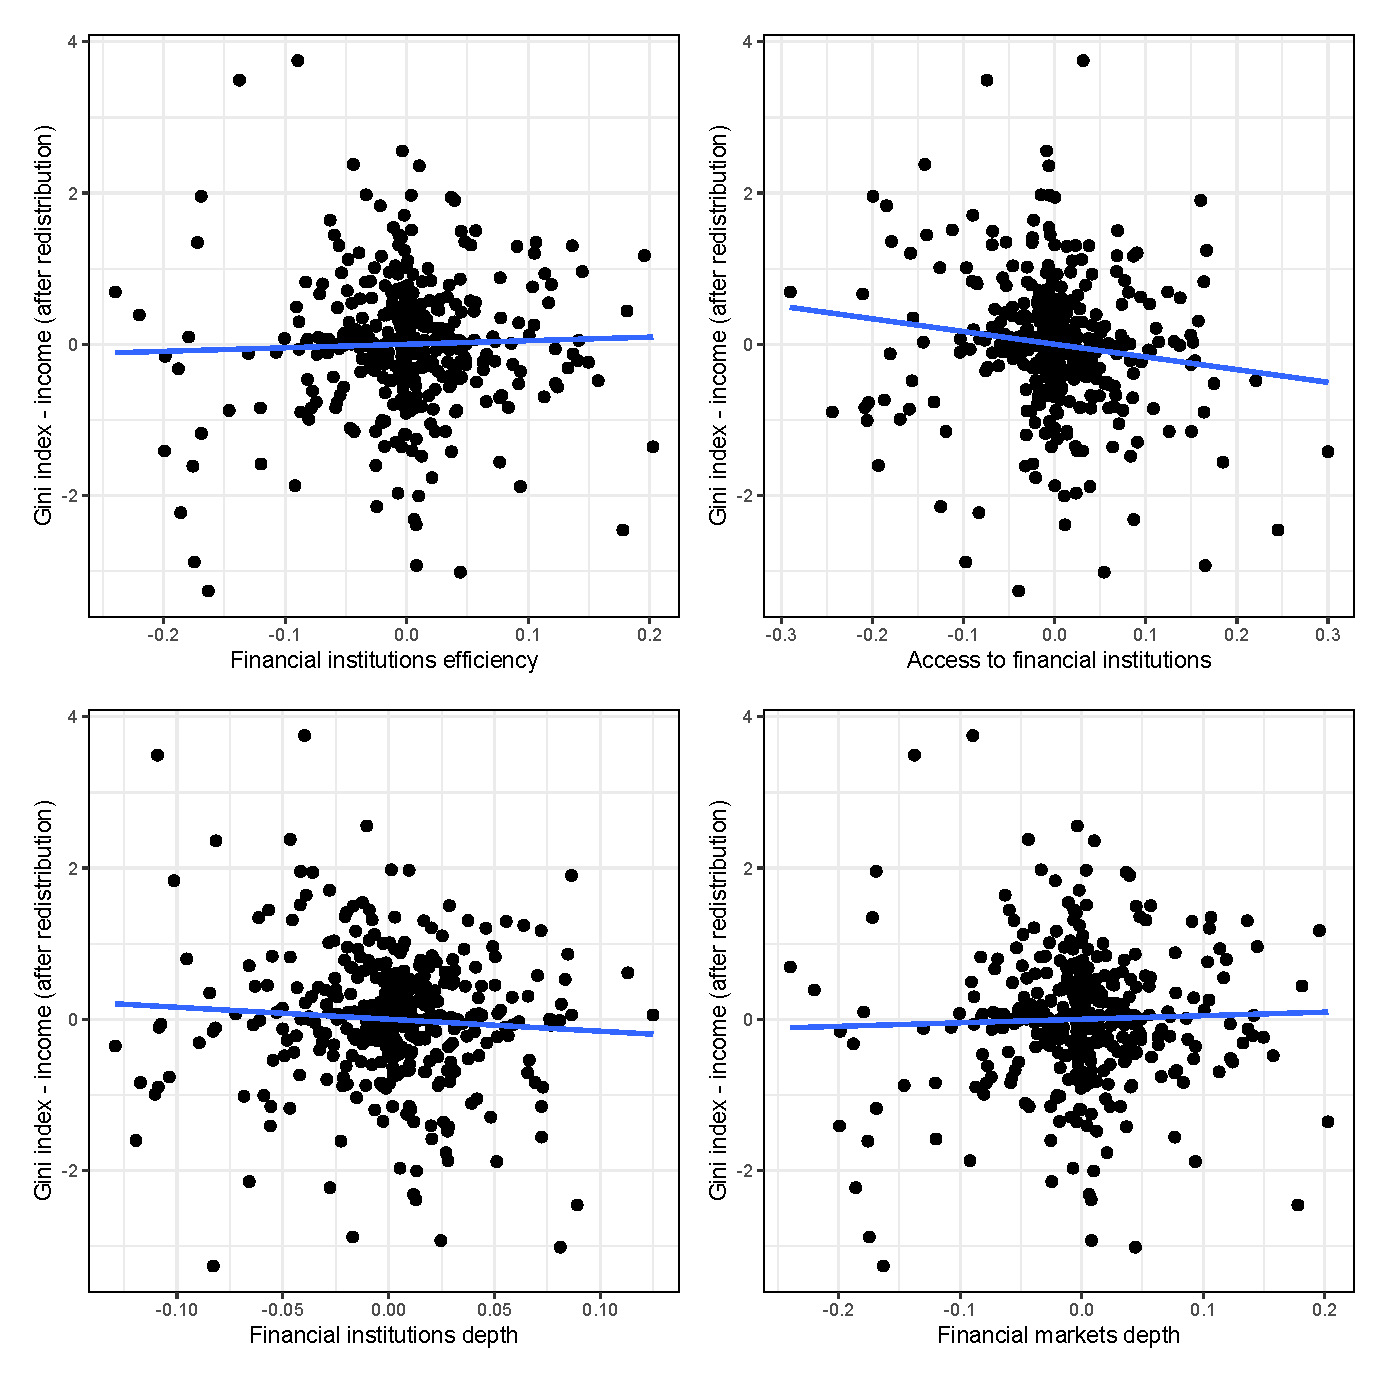
\includegraphics[width=\textwidth, keepaspectratio]{figures/plots_findev_gini_dm}
\end{figure}

%
%
\section{Methodology}
% \label{sec:meth}

\section{Results}
% \label{sec:results}

% \label{sec:conclusion}

\clearpage
%
\bibliographystyle{chicagoa}
\bibliography{literature}
%
\clearpage
%
\appendix
\section{Appendix}
% \label{sec:app}

\renewcommand{\thesection}{A\arabic{section}}%
\renewcommand{\thetable}{A\arabic{table}}%
\renewcommand{\thefigure}{A\arabic{figure}}%
\renewcommand{\theequation}{A\arabic{eq}} 

\end{document}